\chapter{Results}
For monitoring and understanding better the training process, some performance and loss measures were taken into account in generating graphs. 

The relevant performance measures are the length of the episode, accumulated reward, and the value function result. These values should be growing. The length of the episode grows until the agent has been trained to drive the whole lap. The more the car stays in the game and the better it drives, the more reward it gets and the better value function results. If the car crashes then the length of the episode is short, and because it is learning, the graph should show an increasing curve as the training advances. 

The loss measures are the ones that participate in the composition of the loss function. These include policy, value, and entropy losses. These results should show decreasing curves as the loss is being minimized with each step and the estimations become more accurate. The entropy is representing the amount of exploration that the agent is making, the more it learns, the less it explores, and acts more based on his knowledge.

The following figure presents the results of training an agent using A3C: 4 workers in parallel, the Adam optimizer with the learning rate of $10^{-4}$.
\begin{figure}[H]
	\minipage{0.5\textwidth}
	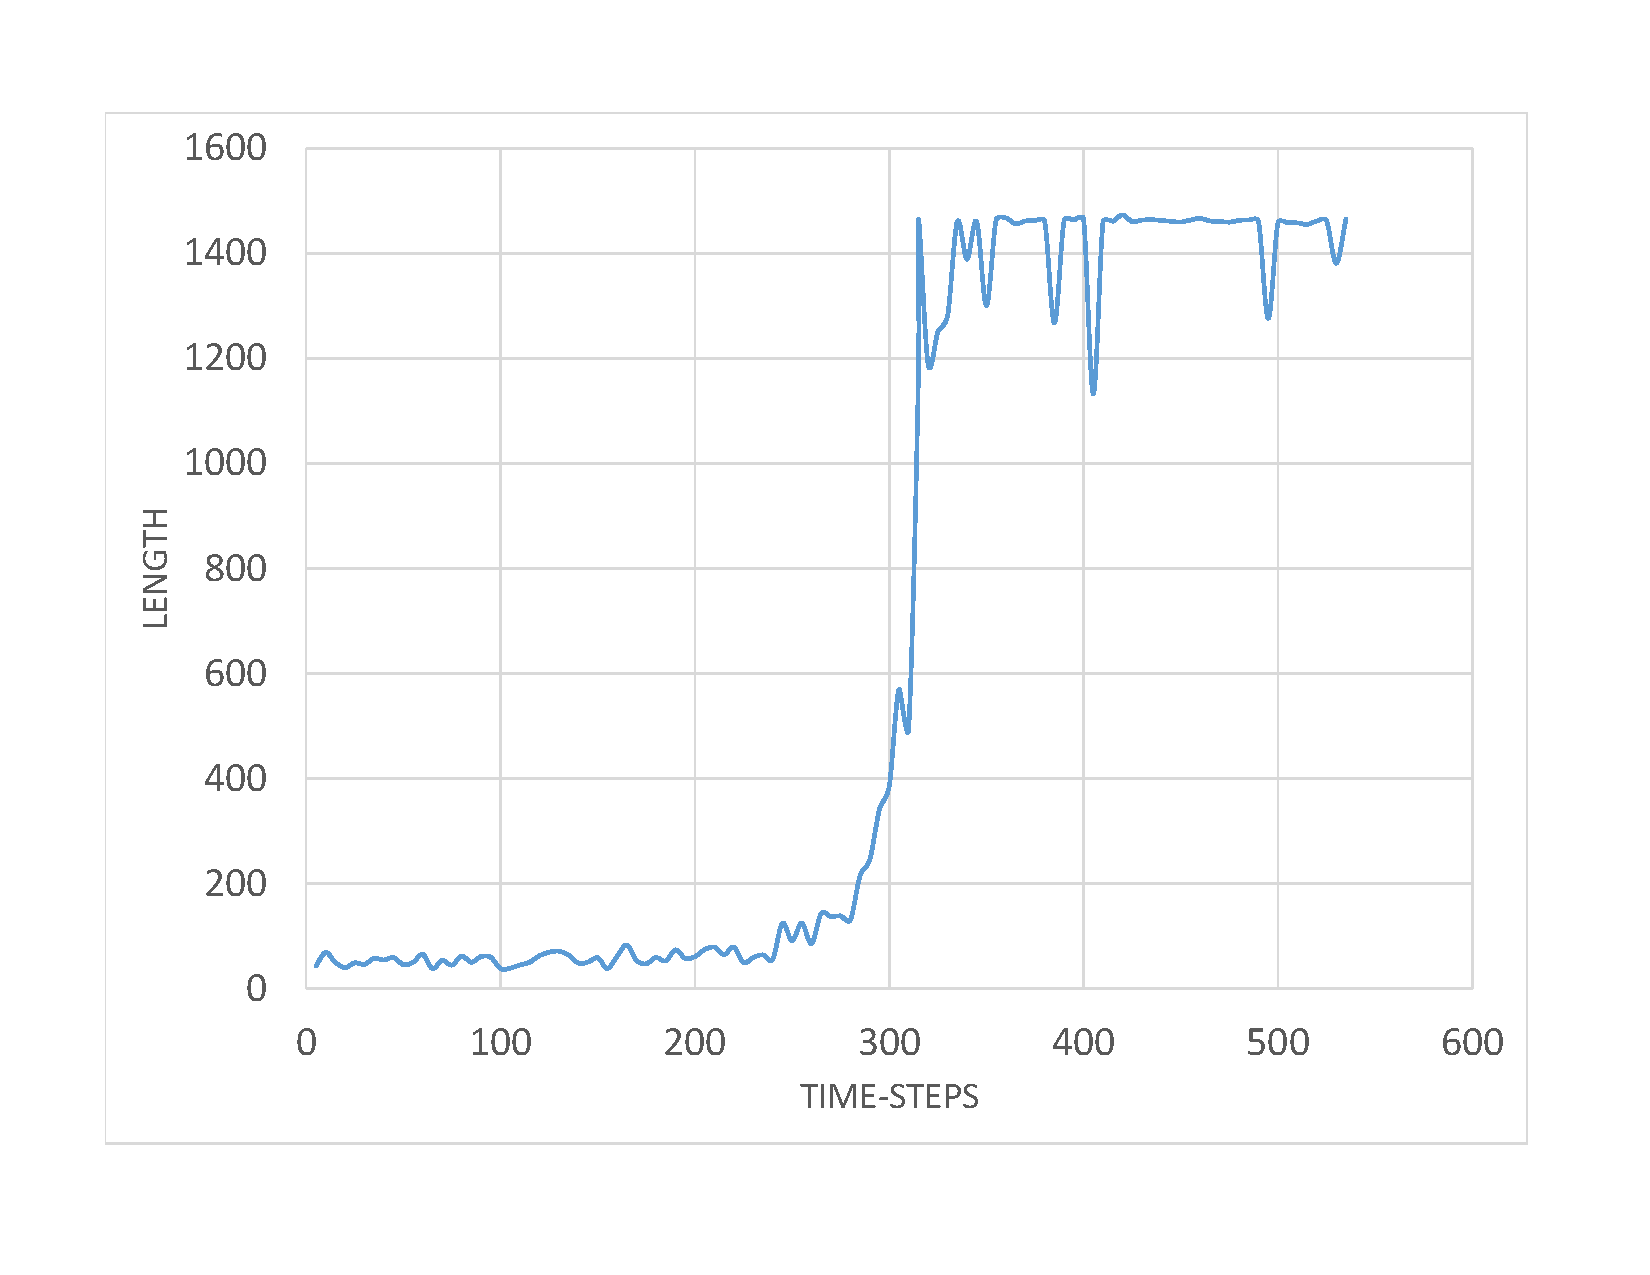
\includegraphics[width=\linewidth]{Figures/Length}
	\caption{Length}\label{fig:Length}
	\endminipage\hfill
	\minipage{0.5\textwidth}
	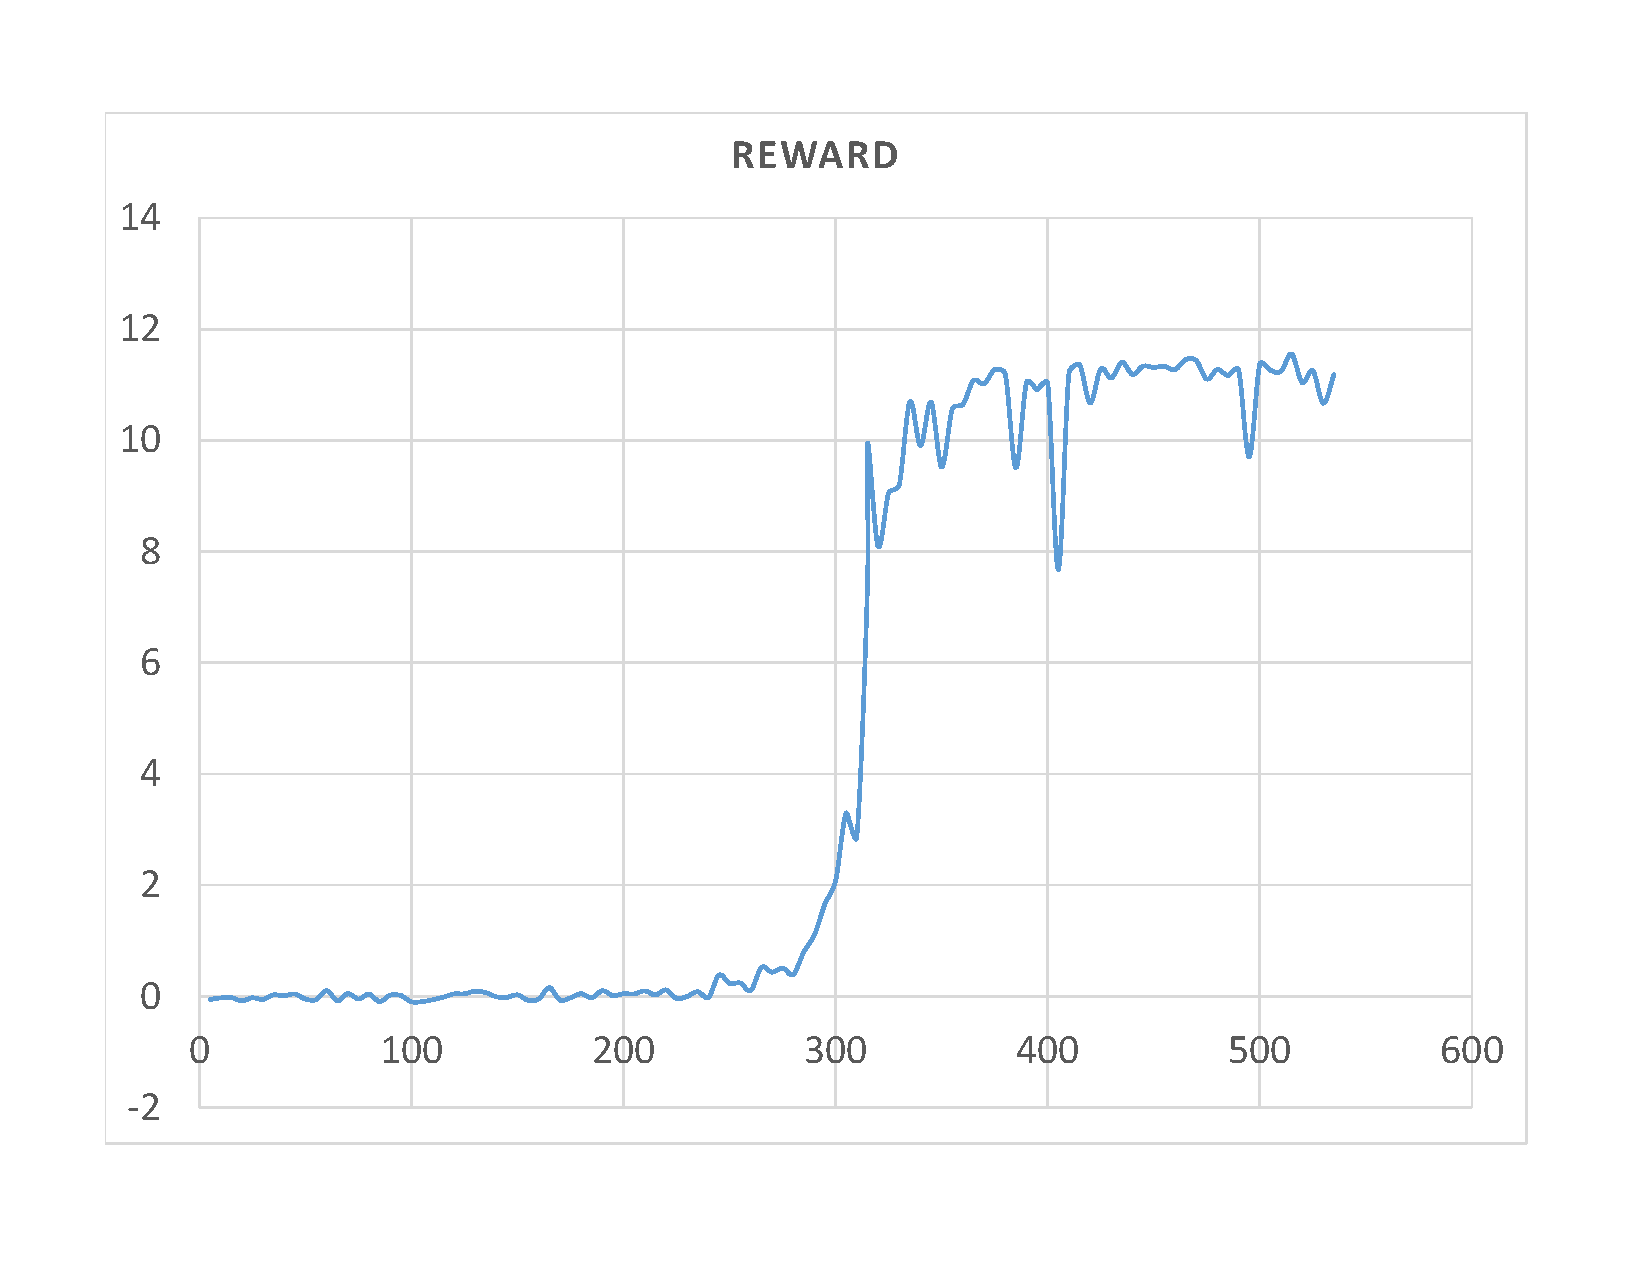
\includegraphics[width=\linewidth]{Figures/Reward}
	\caption{Reward}\label{fig:Reward}
	\endminipage
\end{figure}
\begin{figure}[H]
	\minipage{0.5\textwidth}
	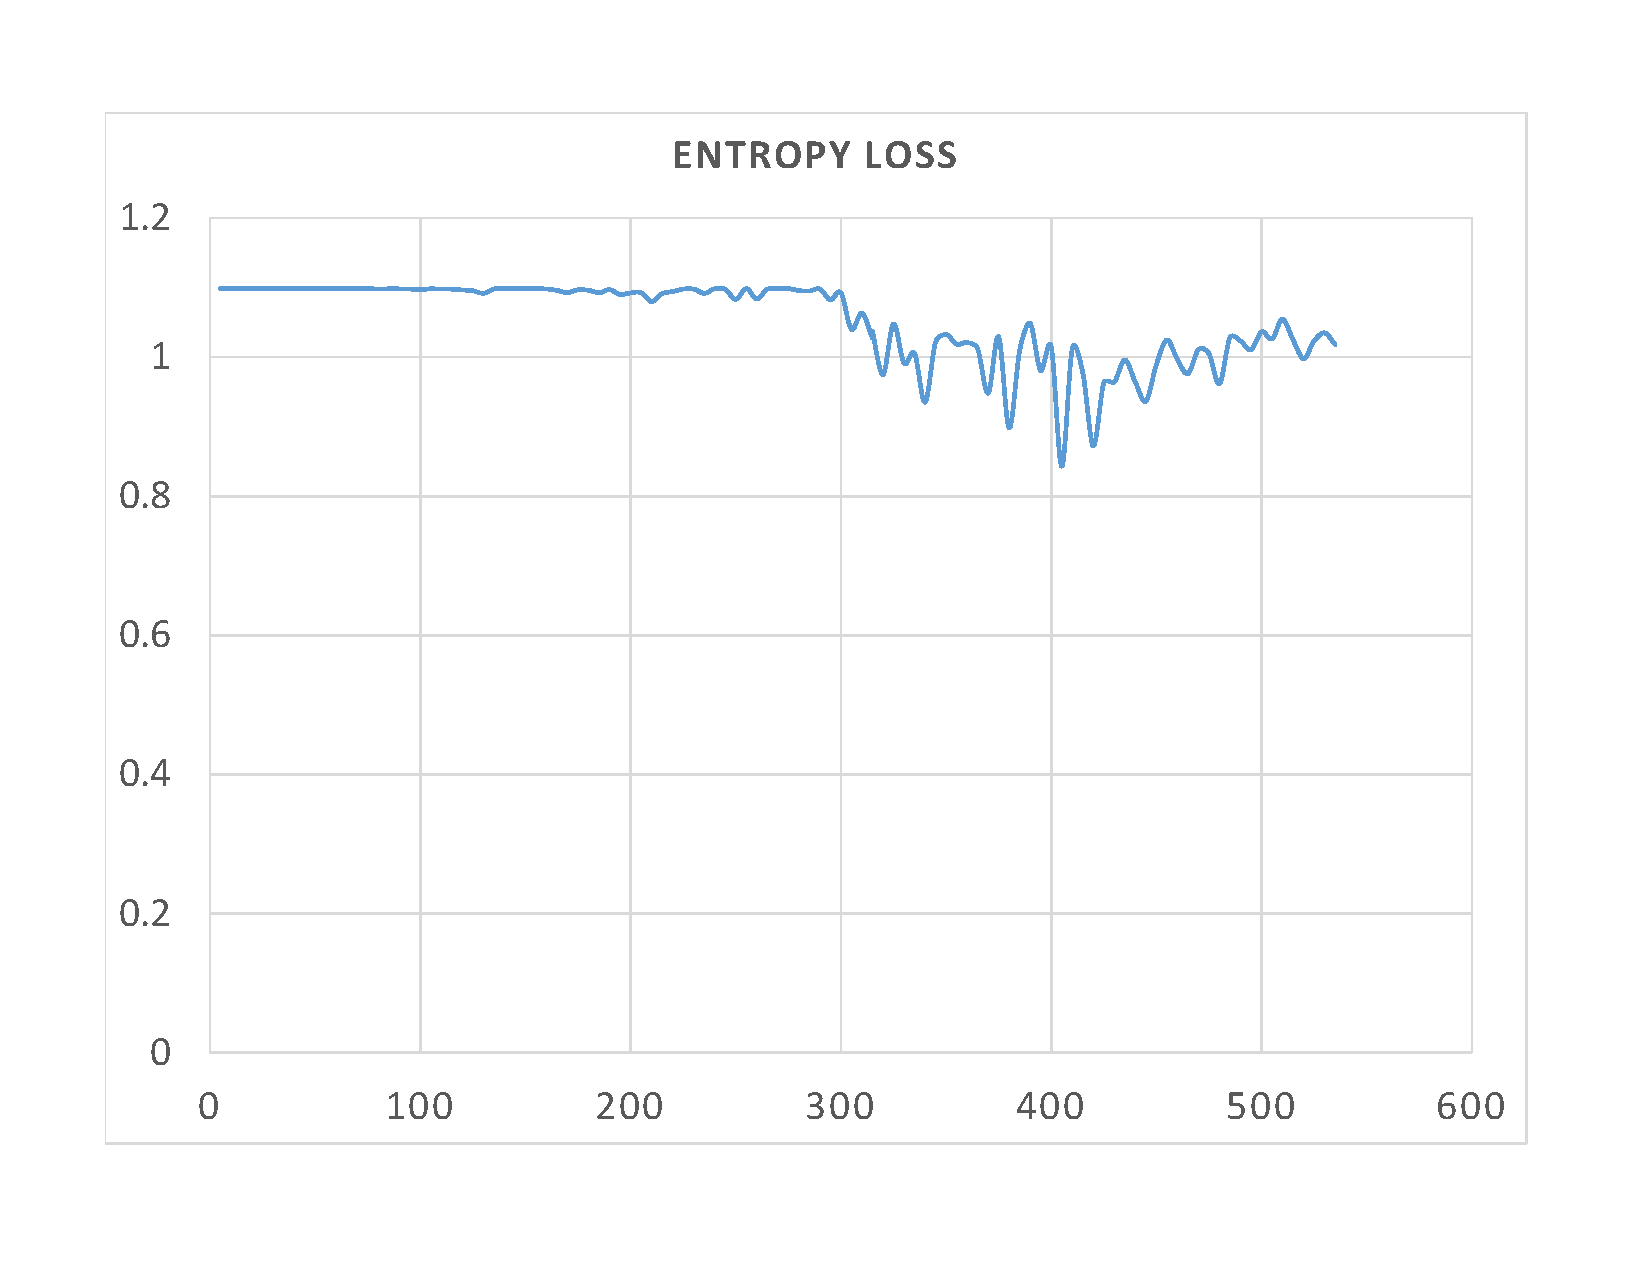
\includegraphics[width=\linewidth]{Figures/EntropyLoss}
	\caption{Entropy Loss}\label{fig:EntropyLoss}
	\endminipage\hfill
	\minipage{0.5\textwidth}
	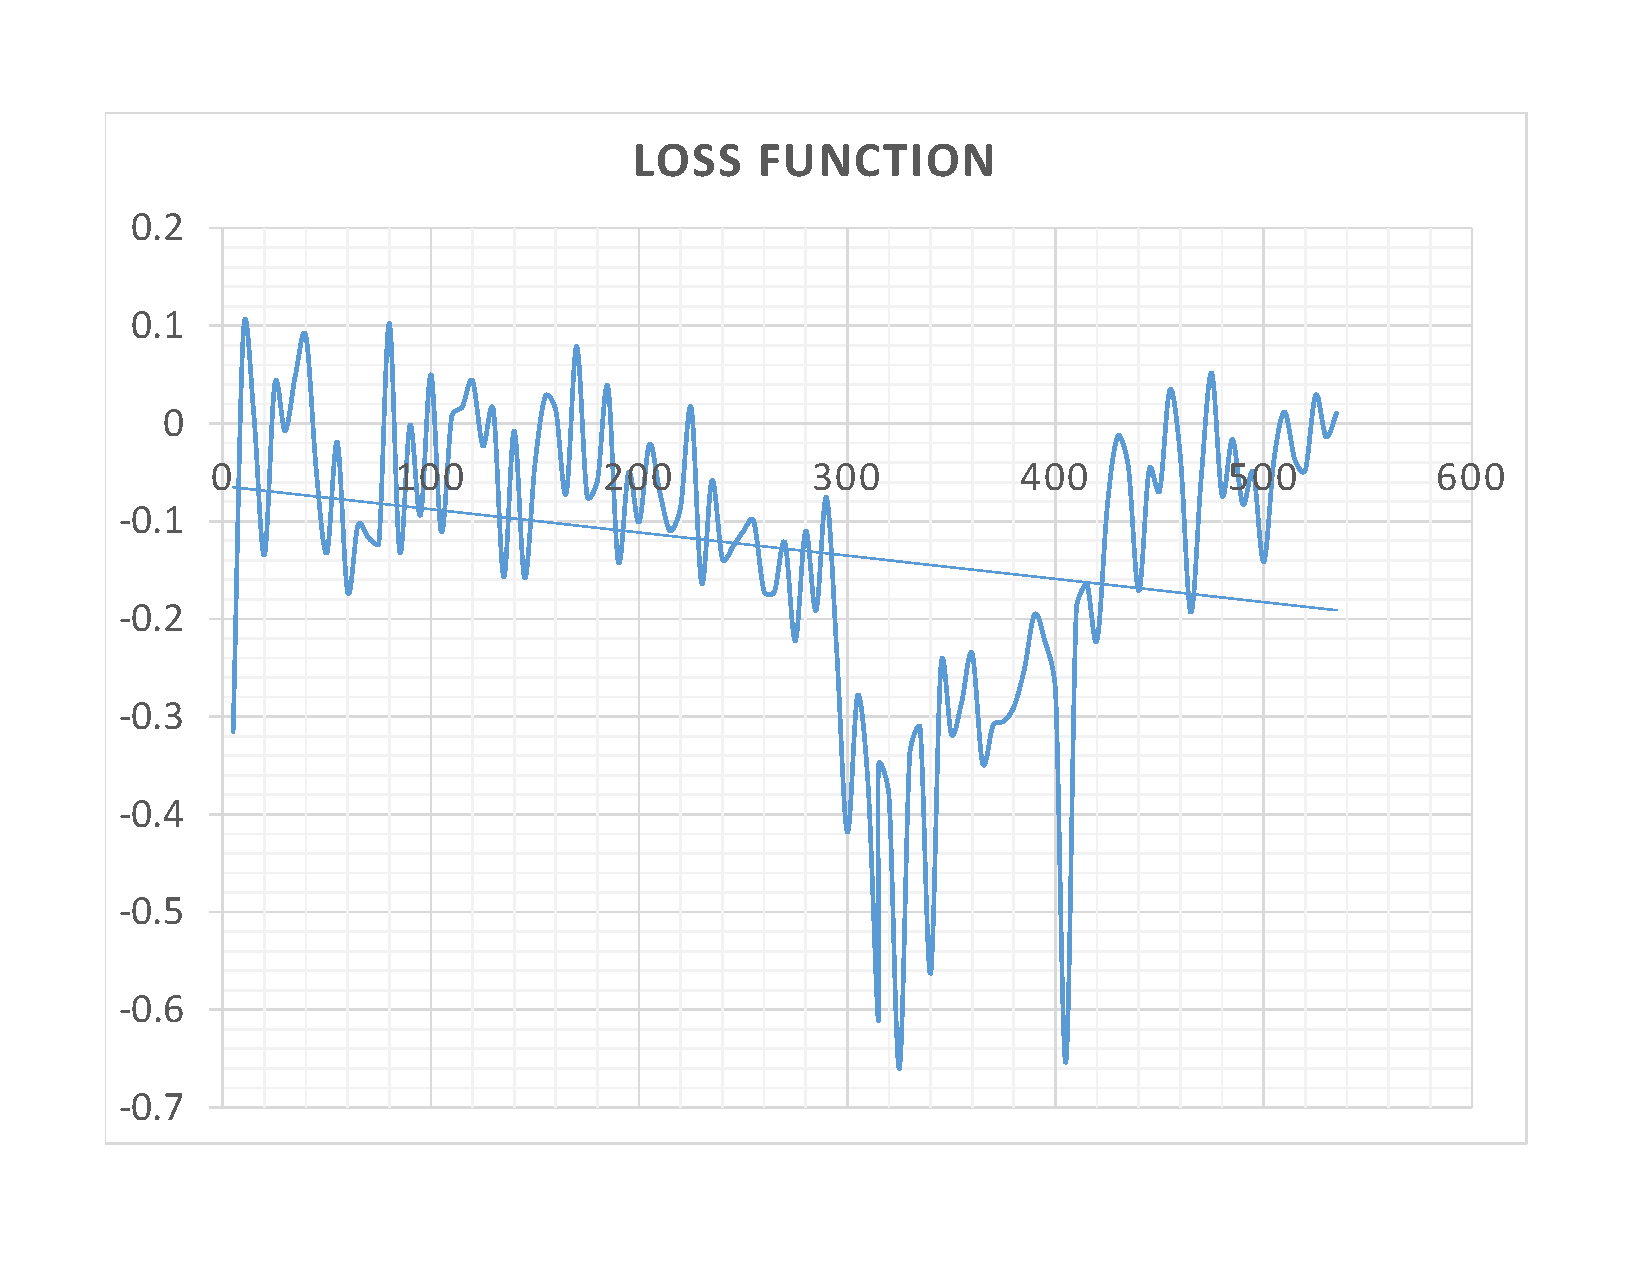
\includegraphics[width=\linewidth]{Figures/Loss}
	\caption{Loss}\label{fig:Loss}
	\endminipage
\end{figure}

As we can see from the figures the training has finished when the agent learned to drive the whole lap and the monotonicity of the plotted curves are as expected (as described above). After $5-6$ hours ($300$ steps) of training the vales started to converge. The trained agent was played on different tracks to test that it learned to drive, but more about this in the section about the different tracks.

The chapter continues with presenting the different scenarios that offer insights in performance and environment manipulations. More precisely, the performance of two different optimizers will be compared, the scenarios with different number of workers will be presented, and different action spaces. The environment specific experiments list some manipulations with the reward function, acceleration and playing the trained agent on other tracks, too.

%network
\section{Optimizers}
It was mentioned at the end of the previous chapter that the recommended optimizers were RMSProp and Adam. RMSProp was used in the experimental set-ups of the Atari games in \cite{DBLP:journals/corr/MnihKSGAWR13} and TORCS in \cite{DBLP:journals/corr/MnihBMGLHSK16}. Also, RMSProp was mentioned in section \ref{RNN} as a solution for the vanishing and exploding gradients problems in RNNs. The Adam optimizer was more often found in the working examples online: in the DDPG for TORCS \cite{DDPG_Torcs}, and in the A3C for Doom \cite{A3CDoom}.

RMSProp and Adam algorithms are extensions of the basic SGD (described in the section \ref{Approximate solution methods}). The problem of identifying a learning rate persists, as it is well known that a too low learning rate results in slow training, whereas a too big learning rate would cause a lot of noise in the objective function so that it would never converge. These SGD extensions try to solve the learning rate problem by adapting it for each of the parameters. 

RMSProp's "idea is to divide the learning rate for a weight by a running average of the magnitudes of recent gradients for that weight" \cite{RMSProp}. The update formula is given by \cite{DBLP:journals/corr/MnihBMGLHSK16}:
\begin{equation}\label{RMSPropUpdate}
\begin{aligned}
g&=\alpha g + (1-\alpha)\Delta \theta^2\\
\theta & \leftarrow \theta - \eta  \frac{\Delta \theta}{\sqrt{g+\epsilon}},
\end{aligned}
\end{equation}
where $\theta$ represents the weights shared across all threads, $\Delta \theta$ is the accumulated gradients of the loss with respect to the $\theta$, $\eta$ is the learning rate, $\alpha$ is the momentum that keeps knowledge of the previous experience, and $g$ is "the moving average of element-wise squared gradients" \cite{DBLP:journals/corr/MnihBMGLHSK16}.

Adam optimizer's principles are a lot like those of RMSProp. Adam algorithm not only keeps the second order moments $g_{t}$, but it also keeps the first order moments $m_{t}$ of the gradients, which are both decayed over time \cite{Optimizers}. The corresponding formulas are listed below:
\begin{equation}\label{Adam}
\begin{aligned}
m_{t+1}&=\alpha_{1} m_{t} + (1-\alpha_{1})\Delta \theta\\
g_{t+1}&=\alpha_{2} g_{t} + (1-\alpha_{2})\Delta \theta^2\\
\hat{m}_{t+1}&=\frac{m_{t+1}}{1-\alpha_{1}^{t+1}}  \\
\hat{g}_{t+1}&=\frac{g_{t+1}}{1-\alpha_{2}^{t+1}}  \\
\theta \leftarrow & \theta - \eta  \frac{\hat{m}_{t+1}}{\sqrt{\hat{g}_{t+1}+\epsilon}}
\end{aligned}
\end{equation}

According to the paper \cite{DBLP:journals/corr/MnihBMGLHSK16}, for the asynchronous deep RL methods like the case of A3C, the RMSProp optimizer with shared weights between threads is more robust and also reduces memory requirements than per-thread weights method. So, shared statistics were used for all the scenarios.

Both RMSProp and Adam optimizers are available in the tensorflow library, and, therefore, were easily tried out and analyzed for the current project, A3C TORCS. A comparison of the two optimizers will be elaborated next, based on the tensorboard graphs generated while training the ANN.
\section{Multi-threading}\label{Multi-threading}
The asynchronous part of the A3C algorithm implies a multiplicity of agents trained simultaneously. The different workers share a global network, but train in separate environments. This means that each worker interacts with its own environment, which is a track he is running on. The worker drives the car in a specified track until it crashes, and another frame starts. In such a way, the workers get to explore more of the same track, while incrementally updating a global shared network. This global network is used and continually updated by all the training workers. This facilitates the process of training in a faster tempo because every worker improves the most recent version of the global network.

The global actor-critic network (ACNetwork) is first declared before the workers. Tensorfow has special dedicated methods for enabling multi-threading, which is the Coordinator. The workers are declared and initialized, after which each of them is assigned to a Thread, where they are started to run their own ACNetwork. The multi-threading process is stopped with join() method when all the workers finished their work.

The following figure shows how much faster the training results to be as the number of parallel workers increases. It was chosen to show the performance of accumulating rewards with 1, 4, and  6 workers training in parallel.
\begin{figure}[H]
	\centering
	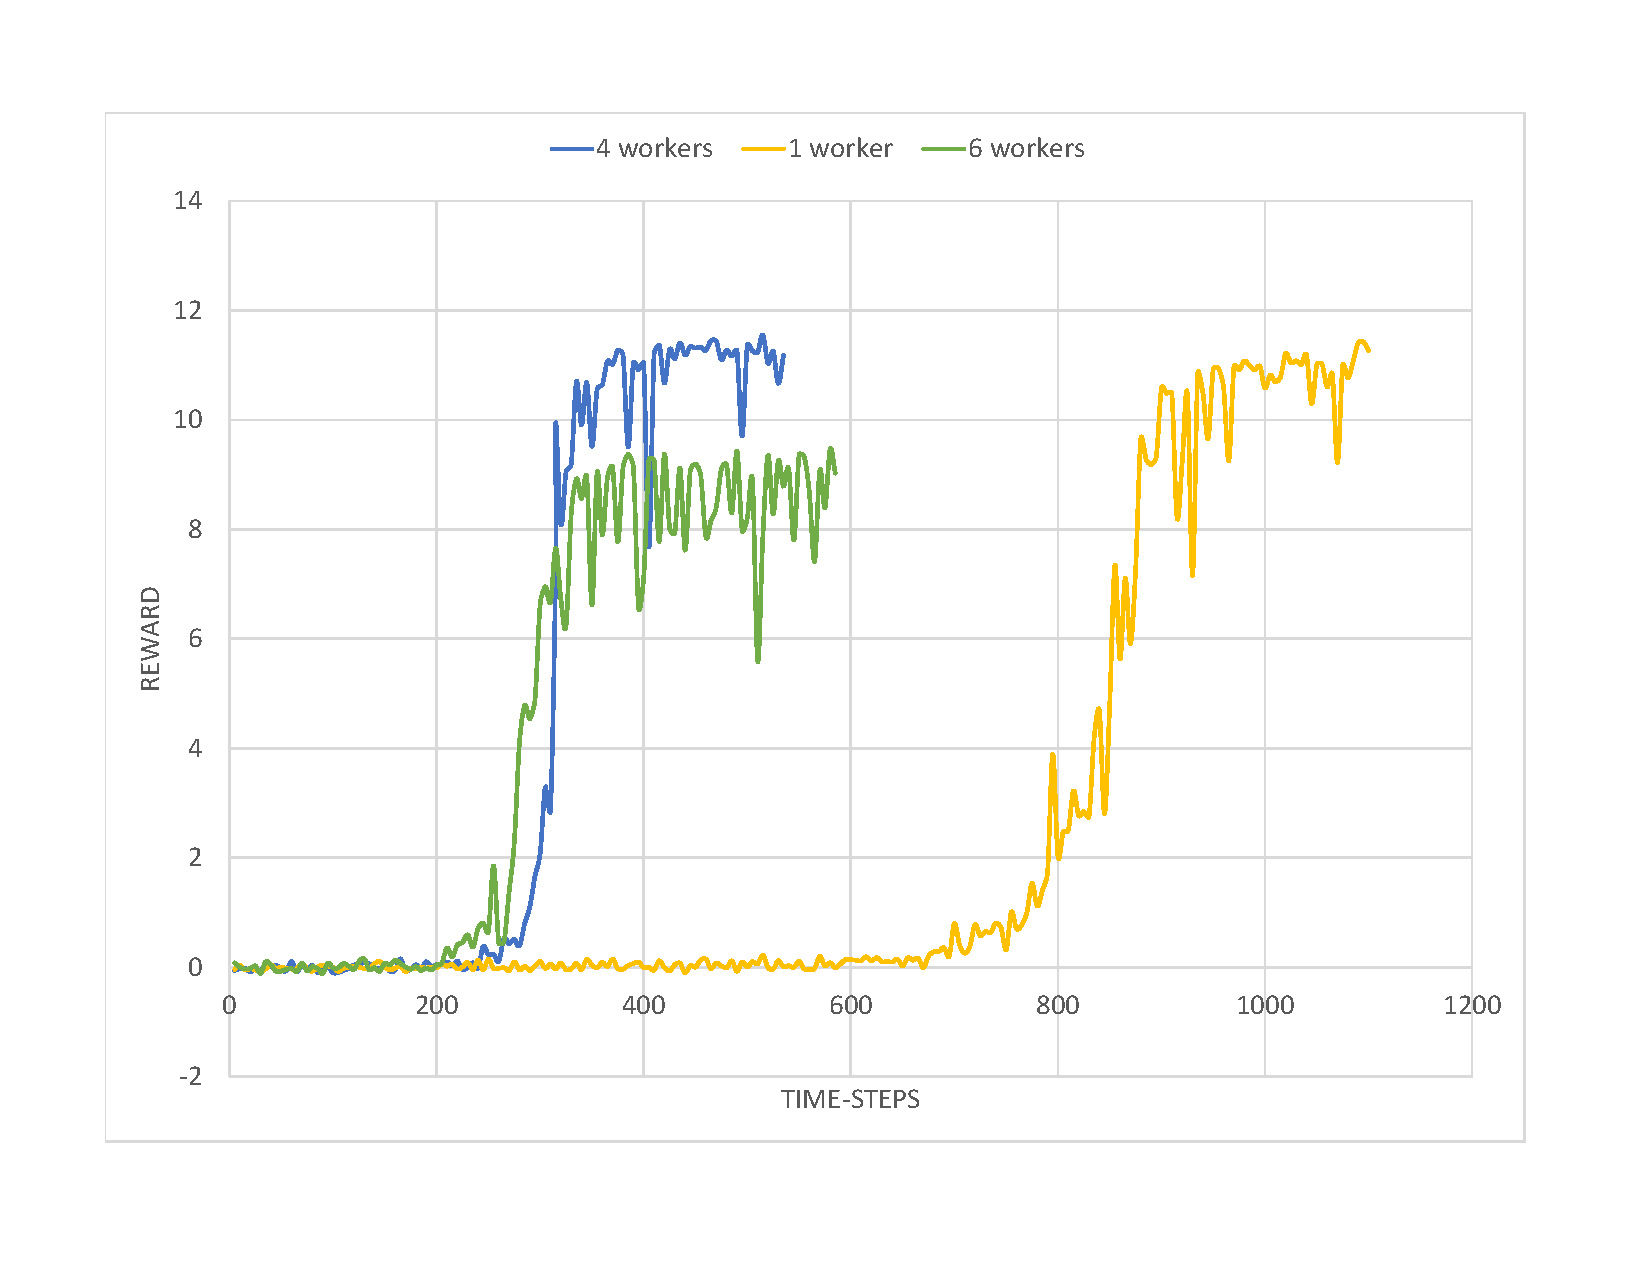
\includegraphics[width=\textwidth]{Figures/Workers}
	\caption{Performance comparison of 1, 4, and 6 workers in parallel}
	\label{fig:Workers}
\end{figure}
 The Figure \ref{fig:Workers} emphasizes that the more workers are used in parallel, the faster the training process becomes. So, for a single worker training alone, the convergence started after 900 time-steps. For 4 workers - the reward function started to grow fast after 250 time-steps, resulting in convergence after 300 time-steps. By increasing the number of workers from 1 to 4, the training became 3 times faster.
 
 It is also possible to see that the training with 6 workers converged to a lower accumulated reward than those of 1 and 4 workers. This is possibly due to a problem of multi-threading the TORCS environment. There are some "Time-out" problems when increasing the number of workers and the performance of the 6 workers was probably affected by it.
\section{Continuous and Discrete Actions Spaces}

\subsection{Discrete Actions Space}

\subsection{Continuous Actions Space}

%environment
\section{Reward}\label{sectionReward}
The reward is really important in reinforcement learning, because it is the one that the agent has to maximize for learning the agent how to act in the environment. For example, consider teaching a dog a new trick: you cannot tell it what to do, but you can reward/punish it if it does the right/wrong thing. It has to figure out what it did that made it get the reward/punishment, which is known as the credit assignment problem \cite{reward_small}. We can use a similar method to train the agent how to drive a car. More about the reward can be read in \Cref{TheorBkgdRL}. 
	
In this project two reward function is compared, for learning the agent how to drive a car in the TORCS environment.  

\subsection*{First reward function}
The first reward function used in this project is the reward function from the paper \cite{DBLP:journals/corr/LillicrapHPHETS15}: \\
\textit{"For the Torcs environment we used a reward function which provides a positive reward each step for the velocity of the car projected along the direction and a penalty of -1 for collisions. Episodes were terminated if progress was not made along the track after 500 frames."}\\
To understand this a figure to illustrate the reward can be seen on \Cref{fig:Reward_paper}.

\begin{figure}[H]
	\centering
	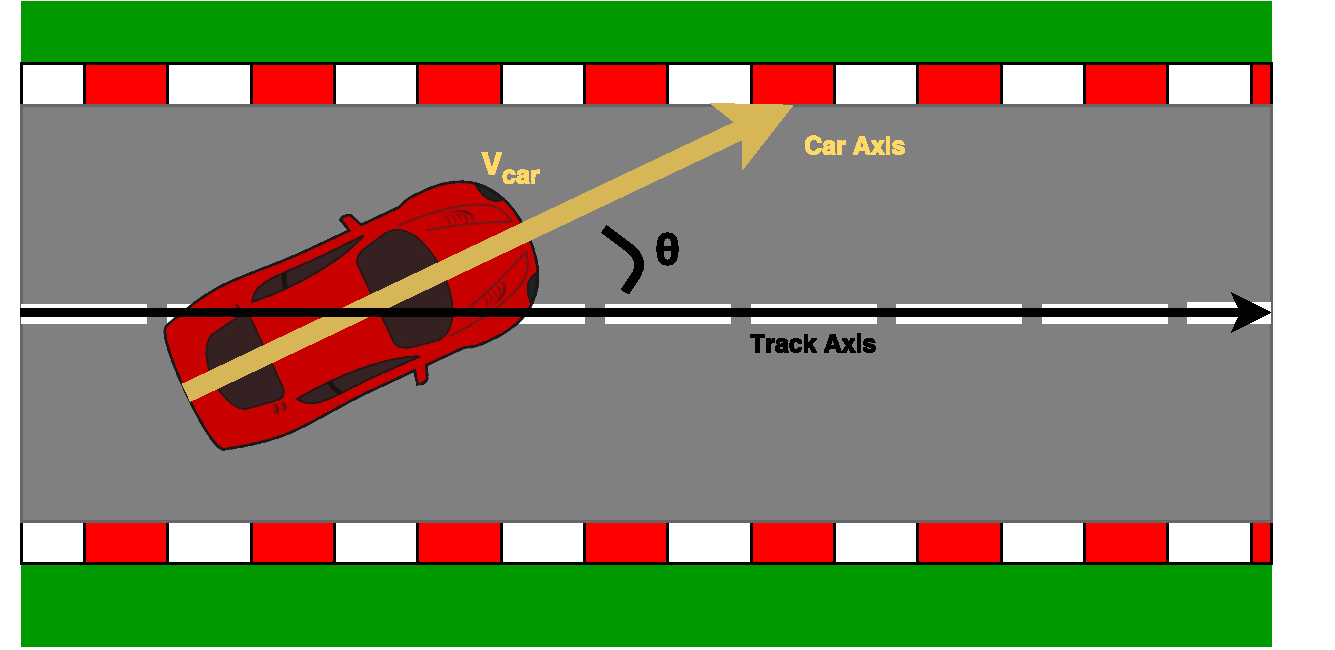
\includegraphics[width=1\textwidth]{Figures/Result/Reward_paper.pdf}
	\caption{Explanation of the reward used in the paper \cite{DBLP:journals/corr/LillicrapHPHETS15} }
	\label{fig:Reward_paper}
\end{figure}

The reward function is then:
\begin{equation}
Reward = V_{car} \cdot cos(\theta) 
\end{equation}
The idea this reward function uses are getting an reward for how fast the car drives in the center of the track. The agent gets more reward, when the car is driving fast at the center of the track, and less reward when the car is driving fast away from the center of the track. 

\subsection*{Second reward function}
After using the first reward function it was concluded that this reward function didn't perform as expected. Because the reward function is important for learning, another reward function is tried. This reward function is taken from the blog \cite{DDPG_Torcs}. Here it uses the same idea, that the reward should be bigger if the car drives fast in the center of the track, and less reward when it is far away from the center. The reward function looks like this:

\begin{equation}
Reward = V_{car} \cdot cos(\theta) - V_{car} \cdot sin(\theta) - V_{car} \cdot \mid trackPos\mid 
\end{equation}
The TrackPos gives percent the car is off center of track. Which is useful in this reward function, when it is wished the car is near the center.  

In this equation the first term want to maximum longitudinal velocity, second term try to minimize transverse velocity, and then it also penalize the AI if it constantly drives very off center of the track in the third term.

Here we see the agent learns how to drive, and this is the reward function where the best results came in this project. It improves the stability of the training.

To test the two reward functions influence on the agent learning, all other parameters stays as described in the introduction to this \Cref{cha:Result}. Thereby it should be possible to only see the influence of the two different reward functions.

To compare both reward functions a graph is created, this graph can be seen on \Cref{fig:change_of_Reward_reward_graph}:

\begin{figure}[H]
	\centering
	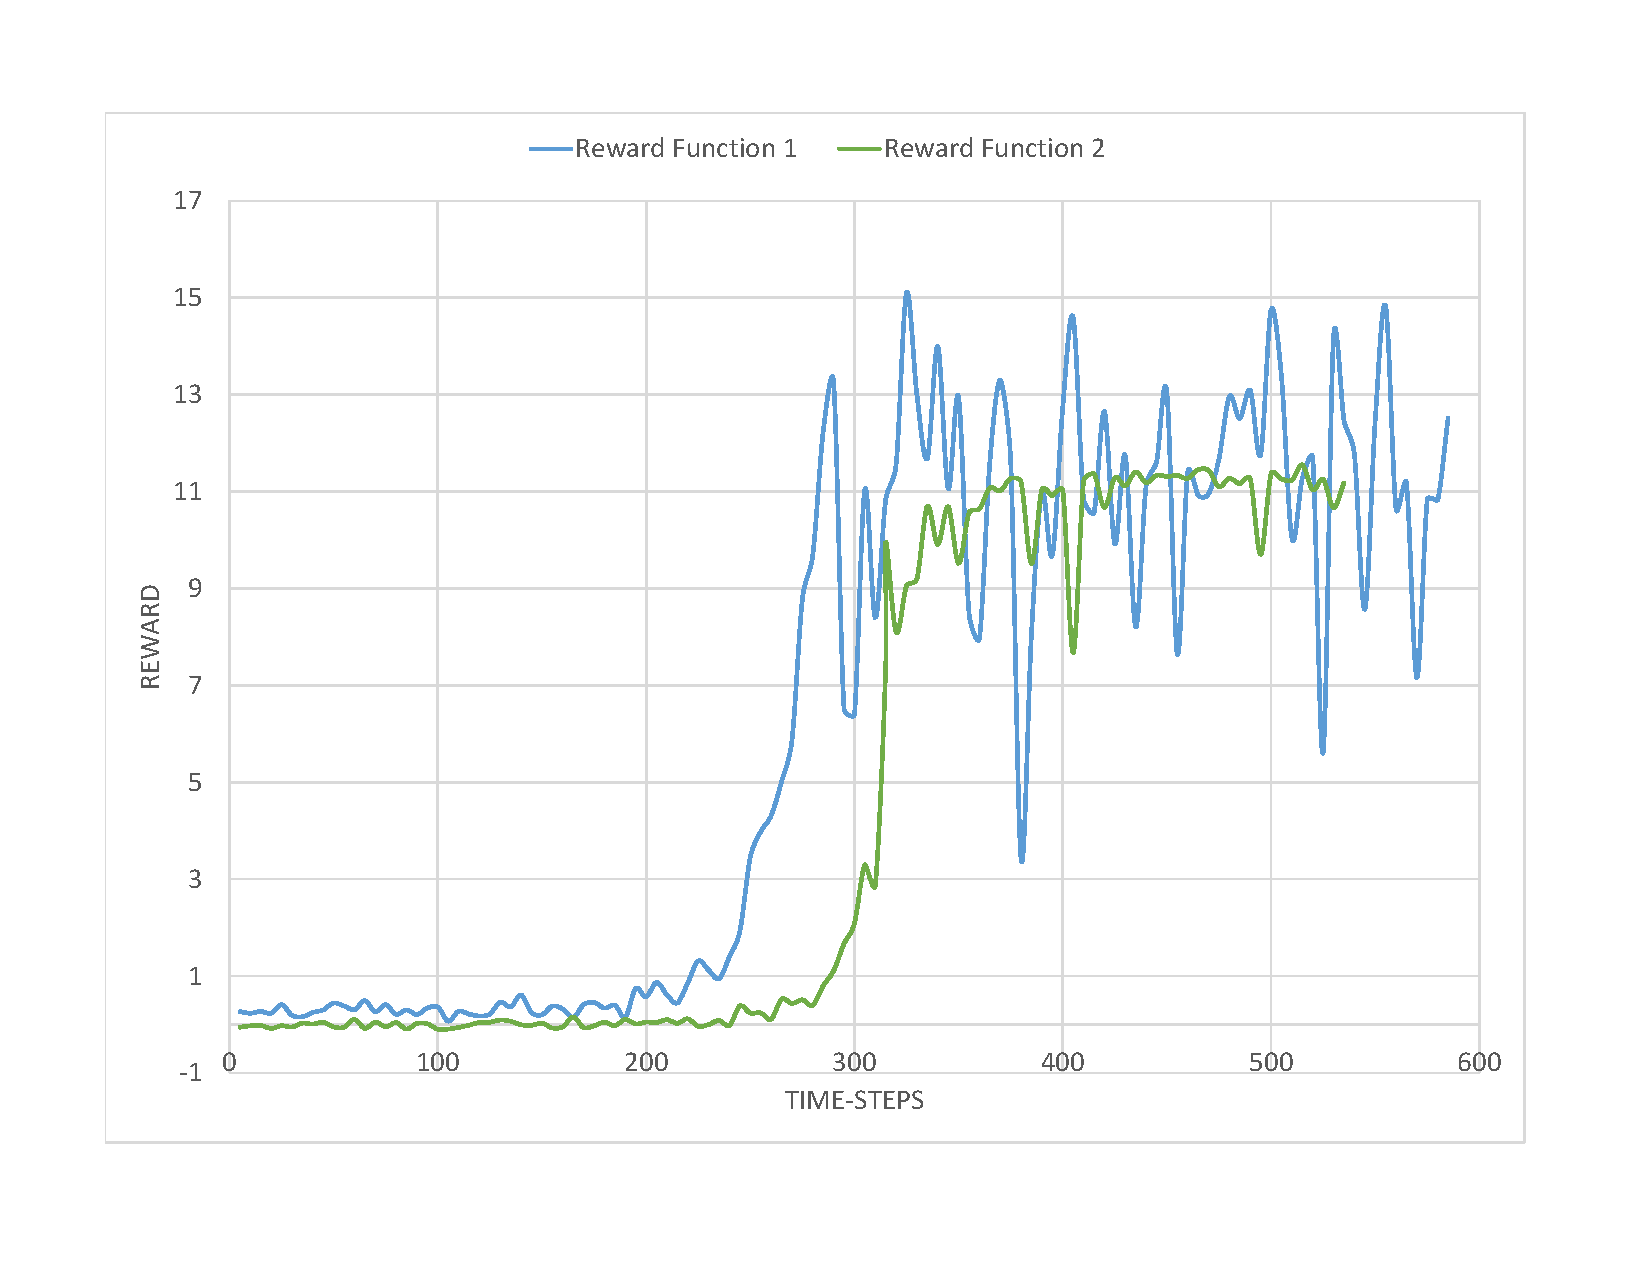
\includegraphics[width=1\textwidth]{Figures/Result/change_of_Reward_reward_graph.pdf}
	\caption{Comparison of the two different reward function with the reward getting from the environment}
	\label{fig:change_of_Reward_reward_graph}
\end{figure}

The \Cref{fig:change_of_Reward_reward_graph} shows the mean total reward of 5 time-steps (episodes). The reward after every step is added together to get the total reward. The total reward is then the reward when an episode is finish. An episode is finished when the car is out of track, the car is driving backwards or the car has finished a lap on the track.  

On the graph on \Cref{fig:change_of_Reward_reward_graph} it is seen that both reward function have the wanted effect, and the first reward function learns a bit faster than the second reward function around 250 time-steps and the second reward function learn around 320 time-steps. The negative side of the first reward function is it is not as stable as the second reward function, by looking at the graphs the second reward function is more stable than the first. 

The stability of the learning can also be seen on the car in the TORCS environment. Here it looks like the first reward function drives close to the edge of the track, and learns how to follow the red and white stripes edges. In the second reward function the car learns to drive better near the center of the road, where the car is more following the white lines in the center of the road. 

The second reward function works best, it is then the reward function which has been used in the final algorithm for the agent.  

\section{Acceleration}
The acceleration is another important parameter in this project. It became important because in the start of the project, the agent has to learn how to accelerate itself. The agent with discrete actions didn't learn the right policy with having the acceleration as an trainable parameter. Acceleration was then changed from an trainable parameter to a constant parameter.

This was done to see if it was possible for the agent to learn how to drive a lap on different speed. This was done because it could be more realistic if it is possible to see the car driving faster than 10 km/h. The tested speed was with an interval of 20 km/h:
\begin{itemize}
	\item 10 km/h
	\item 30 km/h
	\item 50 km/h
\end{itemize} 

The way the car was driving these average speed, was first the car accelerate to a speed of 30 km/h example. After this then accelerating so the speed always stays at 30 km/h. The car will try to stay at this speed 30 km/h the whole lap. To accelerate it is the throttle in the environment which need to be changed.

To test the acceleration influence on the agent learning, all other parameters is as described in the introduction to this \Cref{cha:Result}. Thereby it should be possible to only see the influence on the acceleration.

The most important graph is the graph of the reward, which looks different from all the acceleration, this graph can be seen on {ref to FIGURE reward GRAPH}.


\textbf{FIGURE reward GRAPH}  


On {ref to FIGURE reward GRAPH} it is possible to see what happens with the different accelerations.   
 

  
\section{Tracks}\label{Tracks}
In the TORCS environment is it possible to change the tracks the car is racing in. This is done, to see how it will effect the training. The different tracks is also used for testing. It is possible to test if the car has learned how to drive, by training the car on one track, and then testing it on another track. The car should then be able to drive on both track.  

The setup to test this is the best setup as described in the introduction to this \Cref{cha:Result}. The same setup is then used in all the different track the car has been training on, this is done to make sure that the results from the different track have the same parameters on all the tracks. 

In the environment TORCS there are many different tracks. To get the agent to learn how to drive, a simple track was decided. This was done due to more complicated tracks, had more obstacles like bridges, tress and mountains. A problem with these obstacles is if the agent has to turn left for the first time and it sees many tress there. Then the agent could end up learning it has to turn left every time it sees a tree. then it will take longer for the agent to learn how to drive if there is many obstacles it has to take into account. 

Another issue seen on more complicated tracks is the road the car drives on some times changes through the track also the boundaries of the track can change. This will make it complicated from an agent to learn something, and maybe ending up not learning how to drive. The biggest issue is it will also increase the training time, which will be to long. 

The track shouldn't be to simple, it still has to look like a real road, it also need to have some turns both left and right, so it learns how to drive. 

The track which has been used mostly in this project is a simple track, which have the same road type in the whole track. The track also doesn't have obstacles, only grass around the road, and to boundary from the road to the grass is red and white stripes on the whole track. It has both left and right turns, and also just straight forward, the agent then learn all the different scenarios. The track used mostly in this project can be seen on \Cref{fig:track_simple_1}.

\begin{figure}[H]
	\centering
	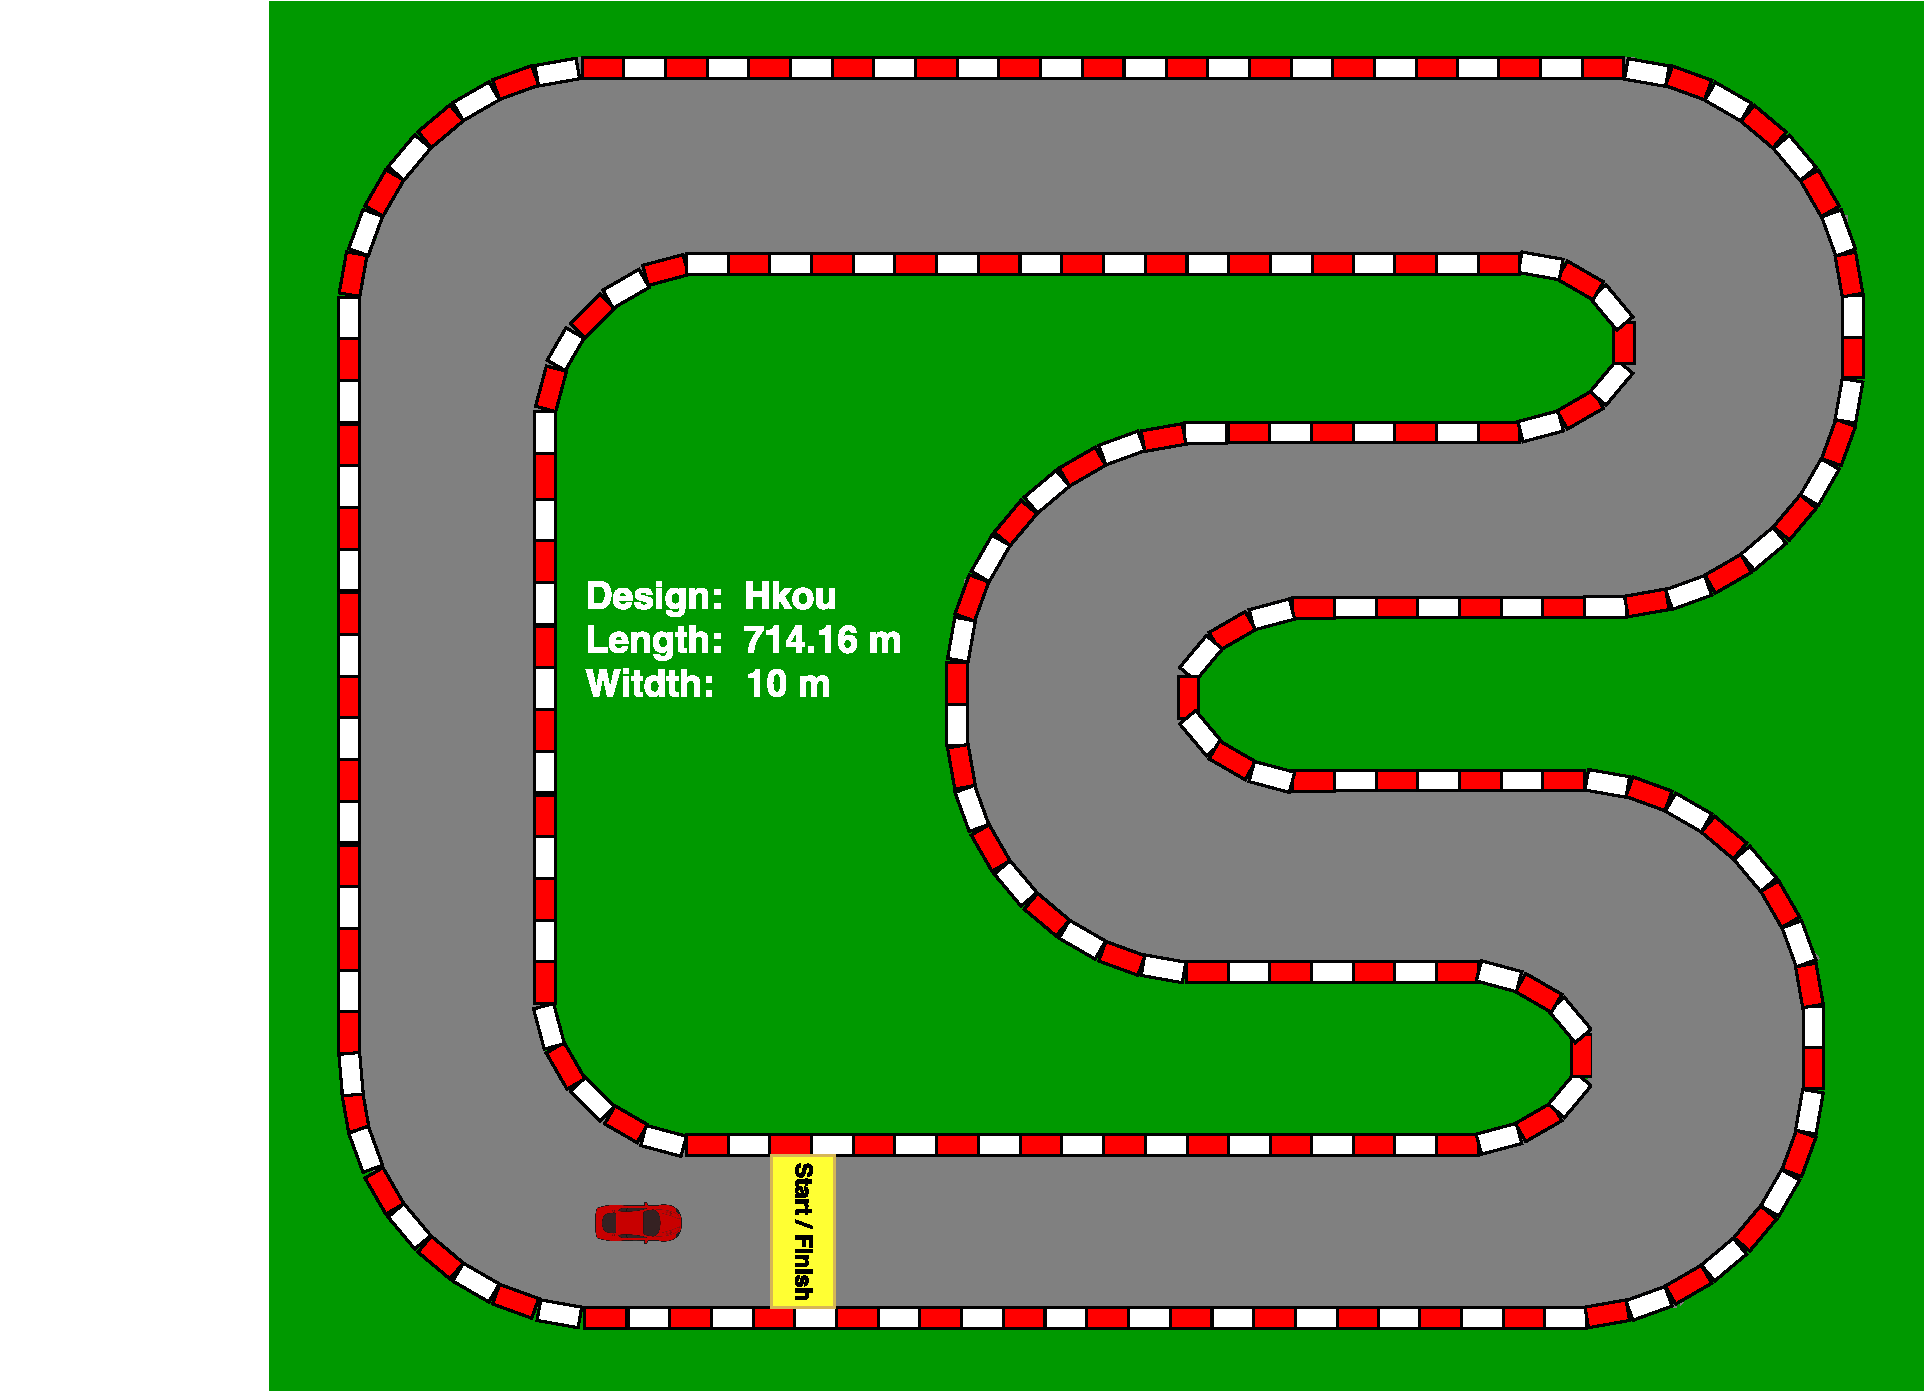
\includegraphics[width=1\textwidth]{Figures/Result/track_simple_1.pdf}
	\caption{The first track used is called $simple\_1$ made by Hkou}
	\label{fig:track_simple_1}
\end{figure}

To find other tracks to train and test on, it has to look similar to the one on \Cref{fig:track_simple_1}, because as mentioned before it learns from the input image. So if it should be possible to test the trained agent, it has to see some of the same things on the test track as on the training track. In the TORCS environment there are three tracks, which look similar the one on \Cref{fig:track_simple_1} and two others. 

The second track used in this project is a track which looks really similar to the first track, and the name is simple\_2 instead of simple\_1. The only difference from the first track is, it is mirrored. This mean that all the turns are exactly opposite. The track is thereby good for testing, because it has different turns than the first track. The second track can be seen on \Cref{fig:track_simple_2}.

\begin{figure}[H]
	\centering
	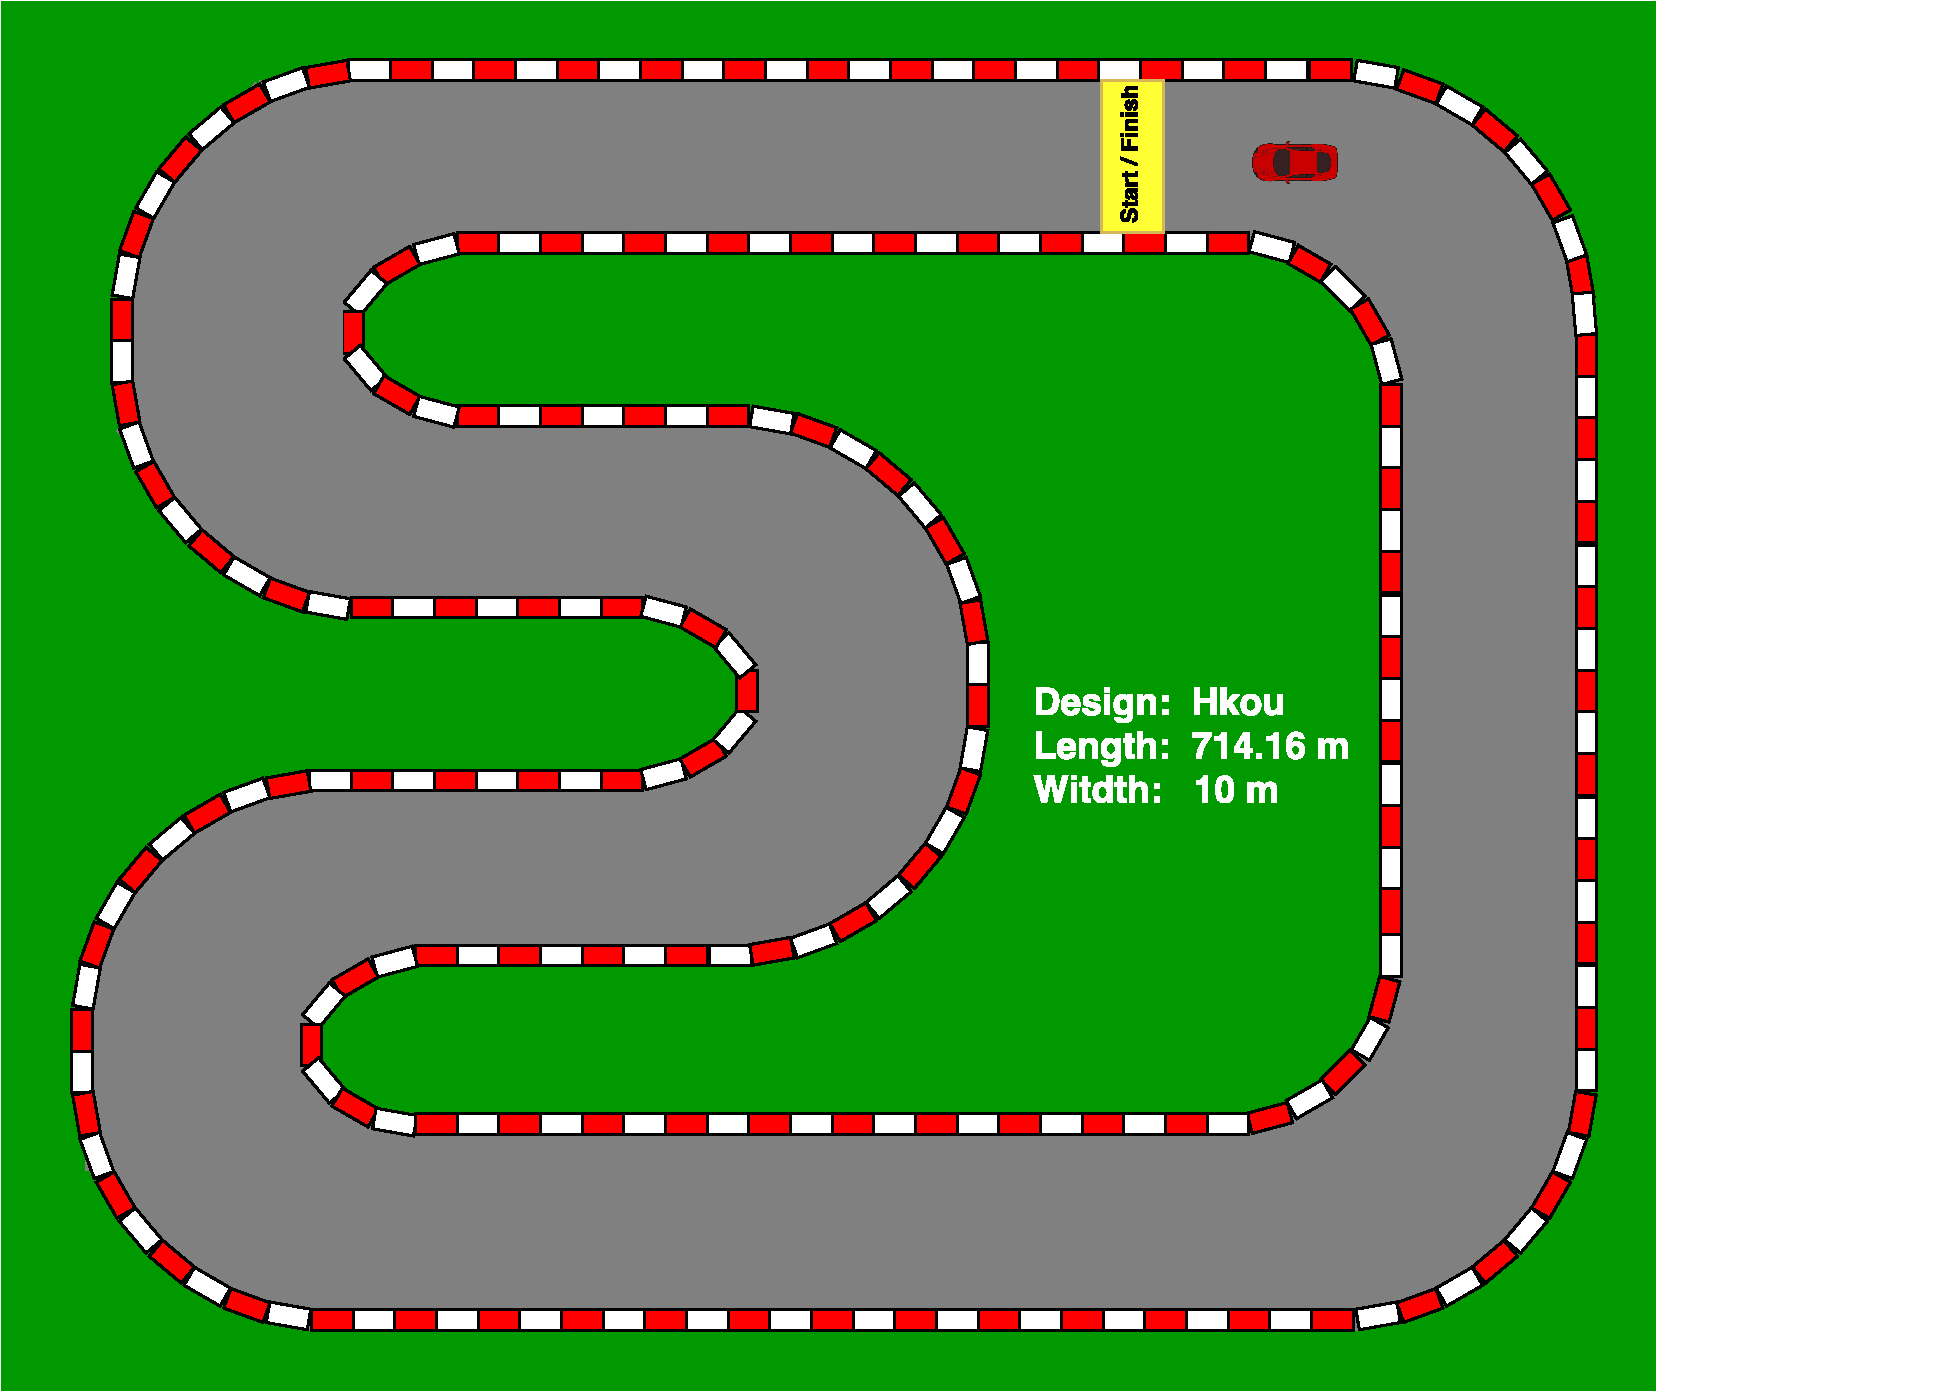
\includegraphics[width=1\textwidth]{Figures/Result/track_simple_2.pdf}
	\caption{The second track used is called $simple\_2$ made by Hkou}
	\label{fig:track_simple_2}
\end{figure}

The last track is similar to the two other tracks on \Cref{fig:track_simple_1} and \Cref{fig:track_simple_2}. The only difference is it is more simple, only has left turns. Another difference form the other two tracks is the length it is much longer than the other tracks. It is because of this length it is used to see how the agent learns on a different track with a longer distance. The last used track in this project can be seen on \Cref{fig:track_longstr}. 

\begin{figure}[H]
	\centering
	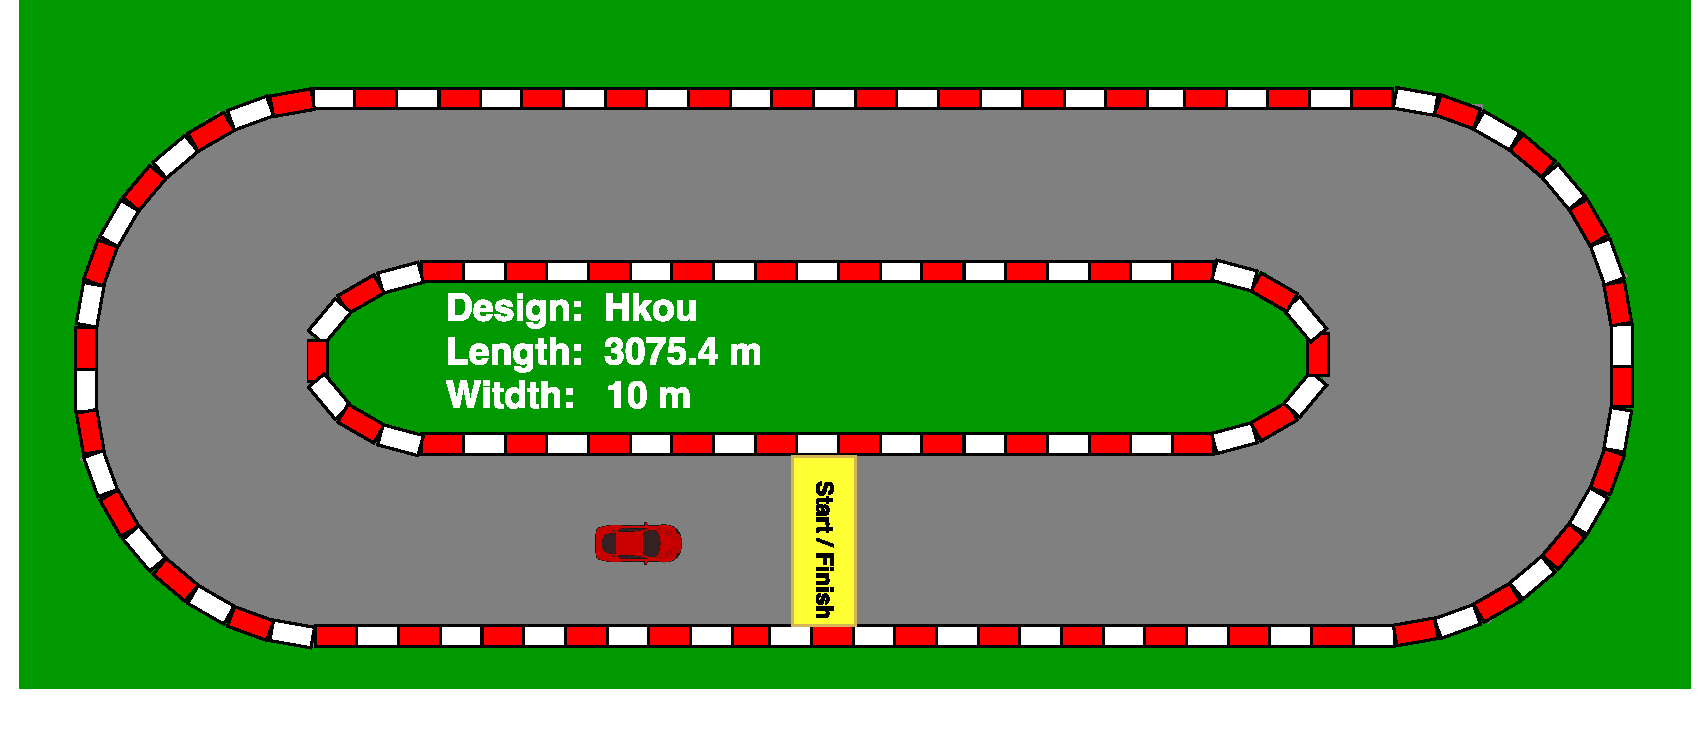
\includegraphics[width=1\textwidth]{Figures/Result/track_longstr.pdf}
	\caption{The third track used is called $longstr$ made by Hkou}
	\label{fig:track_longstr}
\end{figure}


\subsection*{Training}
In this project, it is tested if the tracks has an influence on the training. This is done to see if there is some of the used track which is better to train on than the others.

To compare this training the reward graph is used, the agent has trained on the three different tracks (\Cref{fig:track_simple_1}, \Cref{fig:track_simple_2} and \Cref{fig:track_longstr}). Here it would be better if the reward is growing faster on one of the tracks than the others, and even more important converge to the optimal reward faster. The reward graph can be seen on \Cref{fig:change_of_track_reward_graph}.

\begin{figure}[H]
	\centering
	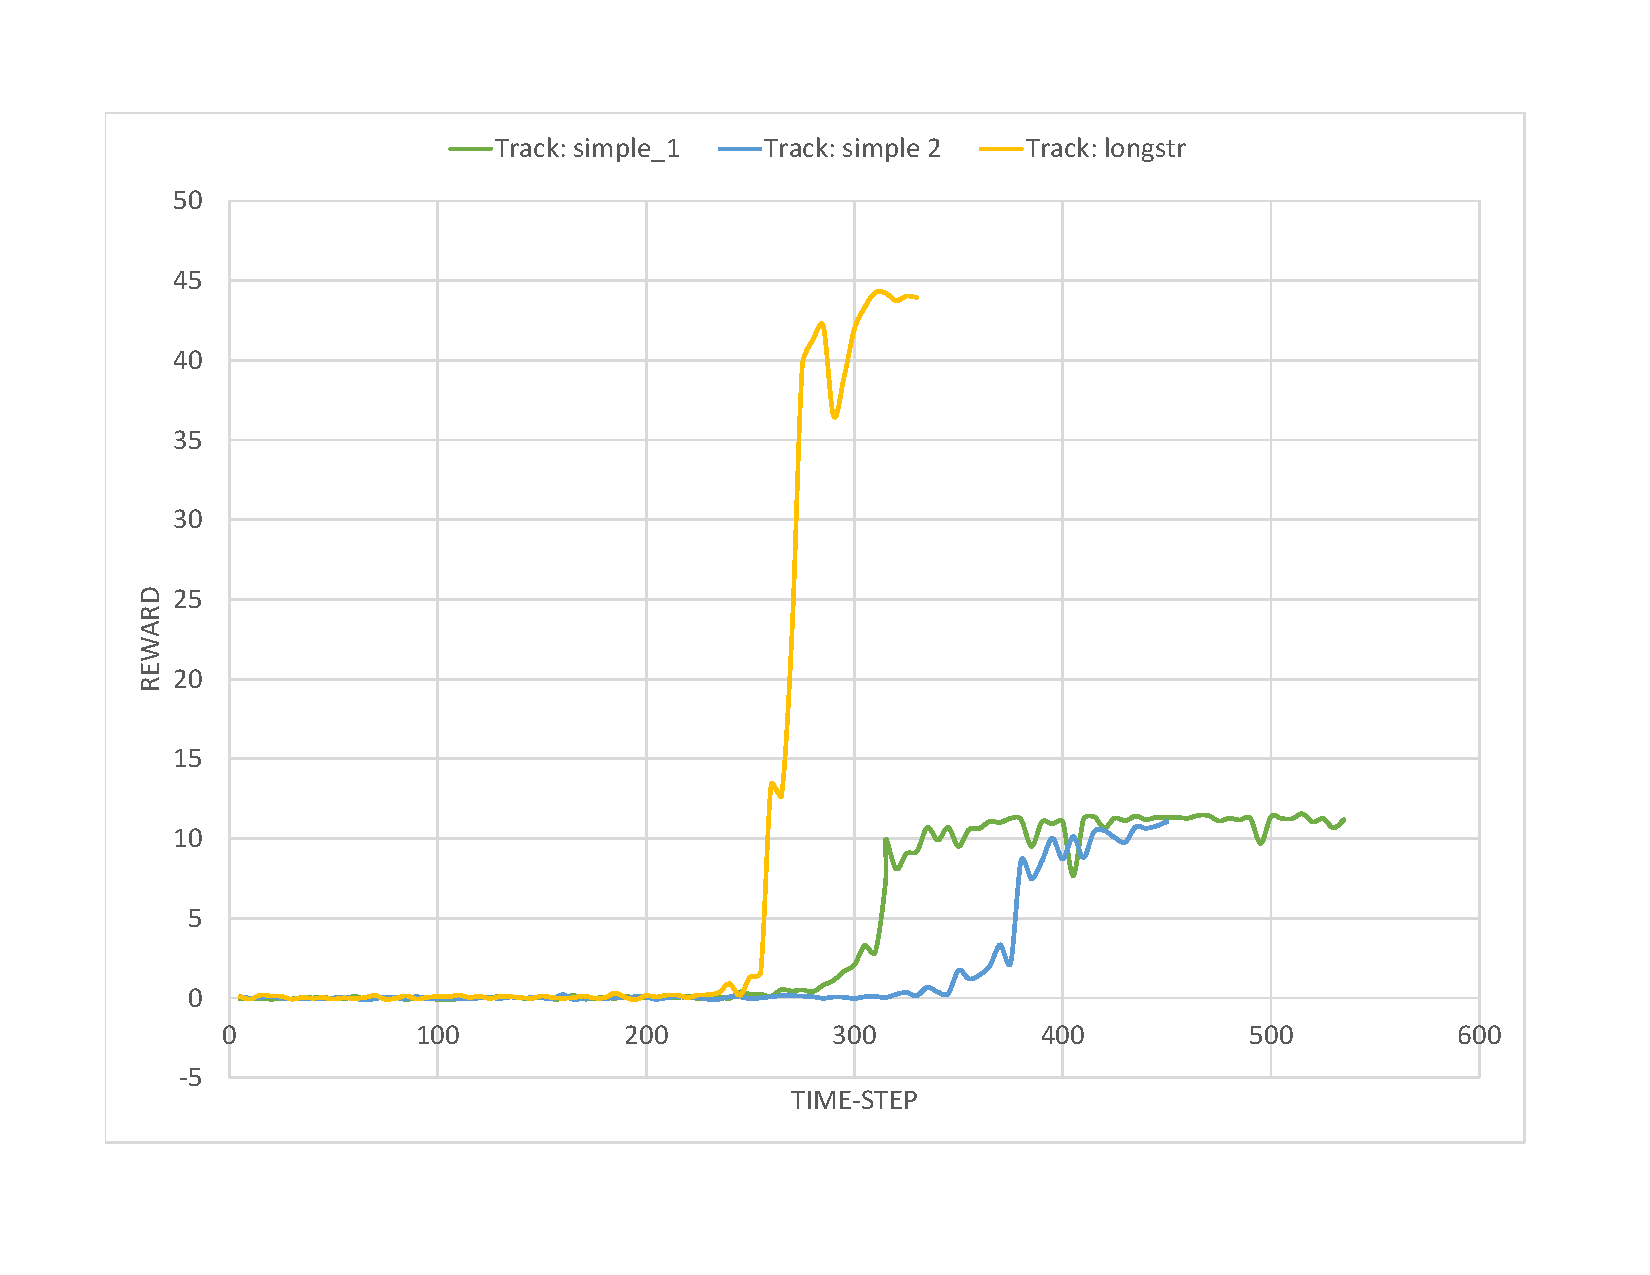
\includegraphics[width=1\textwidth]{Figures/Result/change_of_track_reward_graph.pdf}
	\caption{Comparison of the three different tracks with the reward getting from the environment}
	\label{fig:change_of_track_reward_graph}
\end{figure}

Here it is seen that the different track doesn't have any influence on when the reward starts to grow, they all start around 300 episodes. For the first two tracks which is similar, just mirrored, they have the same graphs. It is as expected, because they have the same length, reward function and acceleration, the training time and reward should then be the same. 

The difference is the reward on the third track, which can be seen to converge to a bigger reward than getting on the two other tracks. This is because of the length of the track. It can get a bigger reward, when the track is longer. This is because the length of every episode is longer. The length of the episodes on the different tracks can be seen on \Cref{fig:change_of_track_length_graph }     

\begin{figure}[H]
	\centering
	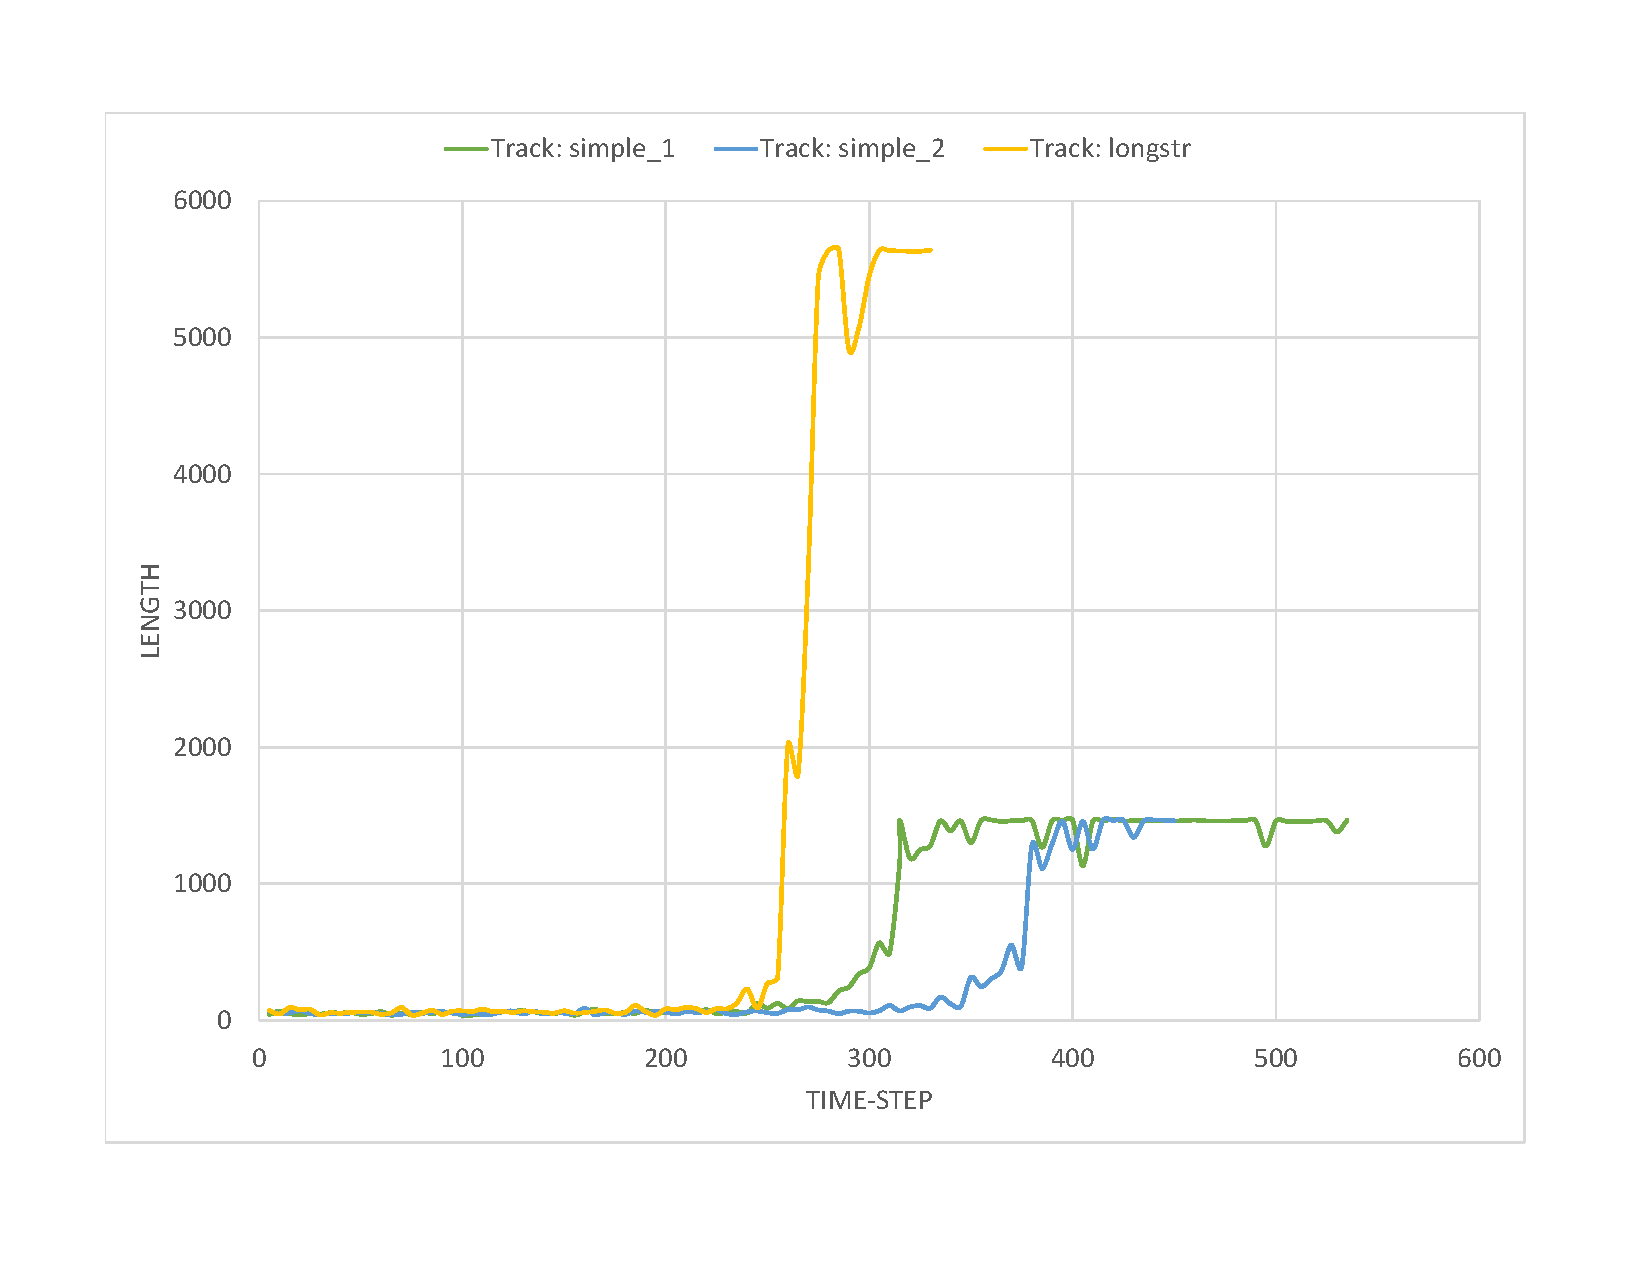
\includegraphics[width=1\textwidth]{Figures/Result/change_of_track_length_graph.pdf}
	\caption{Comparison of the three different tracks with the length of the episodes}
	\label{fig:change_of_track_length_graph}
\end{figure}

Because the track is 3-4 times bigger the reward is also 3-4 times bigger \textbf{formulas of the reward and performance}

After these result the track wich have been used in all the other trainings is the first track seen on \Cref{fig:track_simple_1}. To test if the agent has learned how to drive the second track is used seen on \Cref{fig:track_simple_2}. If the agent is able to complete a lap on both of these tracks it is concluded the agent has learned how to drive.   



